\section{Strategic Outlook and Technology Development Roadmap}
\label{sec:roadmap}

Transitioning sintered regolith bio-infrastructure from terrestrial laboratory validation to operational lunar deployment requires a structured Technology Readiness Level (TRL) maturation strategy\cite{ming1989lunar,fateri2019solar,santomartino2024ecomine}. Current research resides predominantly at TRL 2 to 3, characterized by benchtop sintering of lunar regolith simulants and biological assays on returned Apollo samples\cite{paul2022plants,fateri2019solar}. Maturing these technologies into flight-ready systems requires a three-phase development roadmap aligned with international Artemis and lunar exploration campaigns (Figure~\ref{fig:trl_roadmap} and Table~\ref{tab:trl_roadmap}):

\subsection{Phase 1: Laboratory Formulations and Simulant Validation (2024--2026, \texorpdfstring{TRL 1 $\to$ 3}{TRL 1-3})}
The foundational phase centers on materials characterization and multiphysics process modeling using high-fidelity lunar highland and mare simulants\cite{paul2022plants,chen2024measurement}. Key engineering milestones include mapping complex permittivity and dielectric loss tangents across microwave frequencies ($400\,\mathrm{MHz}\text{--}20\,\mathrm{GHz}$)\cite{chen2024measurement}, optimizing volumetric electromagnetic coupling\cite{lim2019numerical}, and establishing precise cooling curves ($<15^\circ\mathrm{C/min}$) to eliminate thermal-stress-induced microcracking\cite{xi2026multiphysics}. In parallel, multi-generational botanical and fungal assays must verify that sintered porous substrates fully eliminate the transcriptomic stress, ROS bursts, and telomeric DNA lesions observed in raw regolith\cite{paul2022plants,ming1989lunar,barbero2024telomere}.

\subsection{Phase 2: Subscale Flight Testing and In-Situ Demonstrations (2027--2030, \texorpdfstring{TRL 4 $\to$ 6}{TRL 4-6})}
The demonstration phase advances autonomous hardware to relevant spaceflight environments\cite{ming1989lunar,liu2013microwave,cockell2018biorock}. Miniaturized microwave and concentrated solar sintering payloads deployed via Commercial Lunar Payload Services (CLPS) landers will validate vacuum degassing, sintering kinetics, and thermal consolidation directly on the lunar surface\cite{ming1989lunar,hendrix2024reactivity,fateri2019solar}. Concurrently, experiments aboard the International Space Station or orbital variable-gravity centrifuges will evaluate two-phase fluid transport and aeration in sintered ceramics under simulated $1/6\,g$, confirming the pore throat envelope ($30\text{--}60\,\mu\mathrm{m}$) required to prevent capillary hypoxia\cite{ming1989lunar,heinse2007porous}. Automated bioreactor payloads will establish continuous microbial bioleaching kinetics from basaltic minerals under fractional gravity\cite{cockell2018biorock,santomartino2024ecomine,cockell2020microbially}.

\subsection{Phase 3: Operational Habitat Integration and Autonomous Production (\texorpdfstring{$>$2031}{>2031}, \texorpdfstring{TRL 7 $\to$ 9}{TRL 7-9})}
The operational phase achieves full integration within a permanent lunar surface base\cite{ming1989lunar,metzger2023cost,anderson2021lunar}. Automated ISRU manufacturing systems will excavate and classify raw regolith, sinter modular hydroponic troughs, and install them into habitat life-support racks\cite{ming1989lunar,fateri2019solar,metzger2023cost}. The agricultural architecture will connect photoautotrophic crop canopies, saprotrophic mushroom cultivation, and external microbial bioweathering reactors into an interconnected closed loop\cite{ming1989lunar,liu2020bioregenerative,cockell2018biorock}. Incorporating automated $500^\circ\mathrm{C}$ pyrolytic bake-out cycles will enable infinite substrate re-use and $>98.5\%$ water recovery, providing a durable foundation for long-duration human life support on the lunar surface\cite{ming1989lunar,anderson2021lunar,barta1994thermal}.

\begin{figure}[t!]
    \centering
    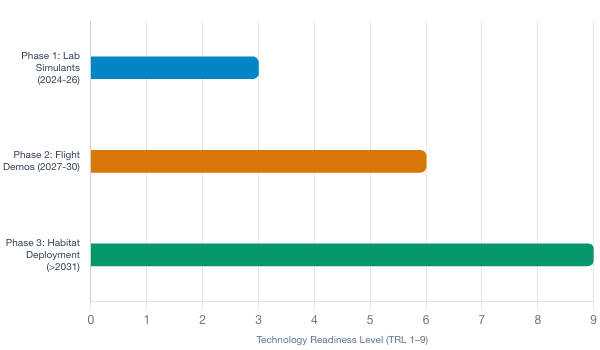
\includegraphics[width=0.85\textwidth]{figures/fig6_trl_roadmap.png}
    \caption{\textbf{Technology Readiness Level (TRL 1--9) maturation horizon for lunar sintered regolith bio-infrastructure.} Strategic progression from Phase 1 laboratory formulations (TRL 1--3, 2024--2026), through Phase 2 subscale flight demonstrations on CLPS landers and the ISS (TRL 4--6, 2027--2030), to Phase 3 operational ISRU habitat integration and closed-loop ECLSS deployment ($>$2031, TRL 7--9).}
    \label{fig:trl_roadmap}
\end{figure}

\begin{table}[t!]
\small
\centering
\caption{\textbf{Strategic technology maturation roadmap for sintered regolith bio-infrastructure.}}
\label{tab:trl_roadmap}
\begin{tabularx}{\textwidth}{lcXX}
\toprule
\textbf{Maturation Phase} & \textbf{Target TRL} & \textbf{Key Technical Milestones} & \textbf{Primary Risks \& Engineering Mitigations} \\
\midrule
Phase 1: Laboratory Formulations (2024--2026) & TRL $1 \to 3$ & Measure dielectric loss tangents across simulants; validate coupled multiphysics models; verify chemical passivation of $\mathrm{npFe}^0$\cite{ming1989lunar,xi2026multiphysics,chen2024measurement}. & \textbf{Risk:} Thermal shock cracking during cooling.\newline \textbf{Mitigation:} Enforce controlled cooling rates $<15^\circ\mathrm{C/min}$\cite{xi2026multiphysics}. \\
\addlinespace
Phase 2: Subscale Flight Testing (2027--2030) & TRL $4 \to 6$ & Deploy autonomous sintering payloads on CLPS landers; validate $1/6\,g$ capillary wicking and gas exchange aboard the ISS\cite{ming1989lunar,fateri2019solar,heinse2007porous}. & \textbf{Risk:} Multiphase fluid separation failure under $1/6\,g$.\newline \textbf{Mitigation:} Constrain pore throat diameters to $30\text{--}60\,\mu\mathrm{m}$\cite{ming1989lunar}. \\
\addlinespace
Phase 3: Operational Deployment ($>2031$) & TRL $7 \to 9$ & Deploy full-scale ISRU manufacturing plant; integrate sintered hydroponics with base ECLSS loops\cite{ming1989lunar,chinnannan2025spirulina,metzger2023cost}. & \textbf{Risk:} Long-term substrate biofouling and pore clogging.\newline \textbf{Mitigation:} Implement cyclic $500^\circ\mathrm{C}$ pyrolytic regeneration\cite{ming1989lunar,santomartino2024ecomine}. \\
\bottomrule
\end{tabularx}
\end{table}
